\documentclass[aspectratio=169]{beamer}
\usepackage[utf8]{inputenc}

\usepackage{amssymb}
\usepackage{amsmath}
\usepackage{graphicx}

\usepackage{listings, xcolor}
\usepackage{bookmark}
\usepackage{hyperref}
% \usepackage{float}
\usepackage{movie15}

\definecolor{codegreen}{rgb}{0,0.6,0}
\definecolor{codegray}{rgb}{0.5,0.5,0.5}
\definecolor{codepurple}{rgb}{0.58,0,0.82}
\definecolor{backcolour}{rgb}{0,0,0}

\lstdefinestyle{mystyle}{
    backgroundcolor=\color{backcolour},   
    commentstyle=\color{codegreen},
    keywordstyle=\color{magenta},
    numberstyle=\tiny\color{codegray},
    stringstyle=\color{codepurple},
    basicstyle=\ttfamily\footnotesize,
    breakatwhitespace=false,         
    breaklines=true,                 
    captionpos=b,                    
    keepspaces=true,                 
    numbers=none,                    
    numbersep=5pt,                  
    showspaces=false,                
    showstringspaces=false,
    showtabs=false,                  
    tabsize=4
}

%%
%% Julia definition (c) 2014 Jubobs
%%
\lstdefinelanguage{Julia}%
  {morekeywords={abstract,break,case,catch,const,continue,do,else,elseif,%
      end,export,false,for,function,immutable,import,importall,if,in,%
      macro,module,otherwise,quote,return,switch,true,try,type,typealias,%
      using,while},%
   sensitive=true,%
%    alsoother={$},%
   morecomment=[l]\#,%
   morecomment=[n]{\#=}{=\#},%
   morestring=[s]{"}{"},%
   morestring=[m]{'}{'},%
}[keywords,comments,strings]%

\lstset{%
    language         = Julia,
    basicstyle       = \ttfamily,
    keywordstyle     = \bfseries\color{blue},
    stringstyle      = \color{magenta},
    commentstyle     = \color{ForestGreen},
    showstringspaces = false,
}

\lstset{style=mystyle}

\usepackage{biblatex} % https://www.overleaf.com/learn/latex/Bibliography_management_in_LaTeX
\addbibresource{main.bib}

% \usepackage{tikz}

% % https://tex.stackexchange.com/questions/40535/matrix-with-arrows-and-labels
% \newcommand{\tikzmark}[1]{\tikz[overlay, remember picture] \coordinate (#1);}

\usefonttheme{serif}
\graphicspath{ {./images/} }

\usetheme[customfont, darkmode]{pureminimalistic} % used the theme: https://github.com/kai-tub/latex-beamer-pure-minimalistic
% \usecolortheme{seahorse}

% removing logo
\renewcommand{\logotitle}{}
\renewcommand{\logoheader}{\vspace{1.5em}}
\renewcommand{\logofooter}{}

% colors 
\definecolor{title}{RGB}{0, 172, 255}
\renewcommand{\beamertitlecolor}{title}


%------------------------------------------------------------
%This block of code defines the information to appear in the
%Title page
\title[Discovering governing equations from data] %optional
{Discovering governing equations from data by sparse identification of nonlinear dynamical systems}

% \subtitle{}

\author[Theo Rode] % (optional)
{Theo Rode}

\date % (optional)
{April 24, 2024}



\begin{document}

%The next statement creates the title page.
\frame{\titlepage}



\section{Background}

% \begin{frame}
% \frametitle{Dynamical Systems}
% \begin{columns}

% 	\column{0.5\textwidth}
% 	\begin{center}
% 		\includegraphics[width=0.95\textwidth, trim = {5pt, 5pt, 5pt, 5pt}, clip]{Examples/slide1_lorenz_attractor.png} % from: http://5010.mathed.usu.edu/Fall2018/ABailey/Lorenz%20Attractor%20.html
% 	\end{center}

% 	\column{0.5\textwidth}
% 	\begin{center}
% 		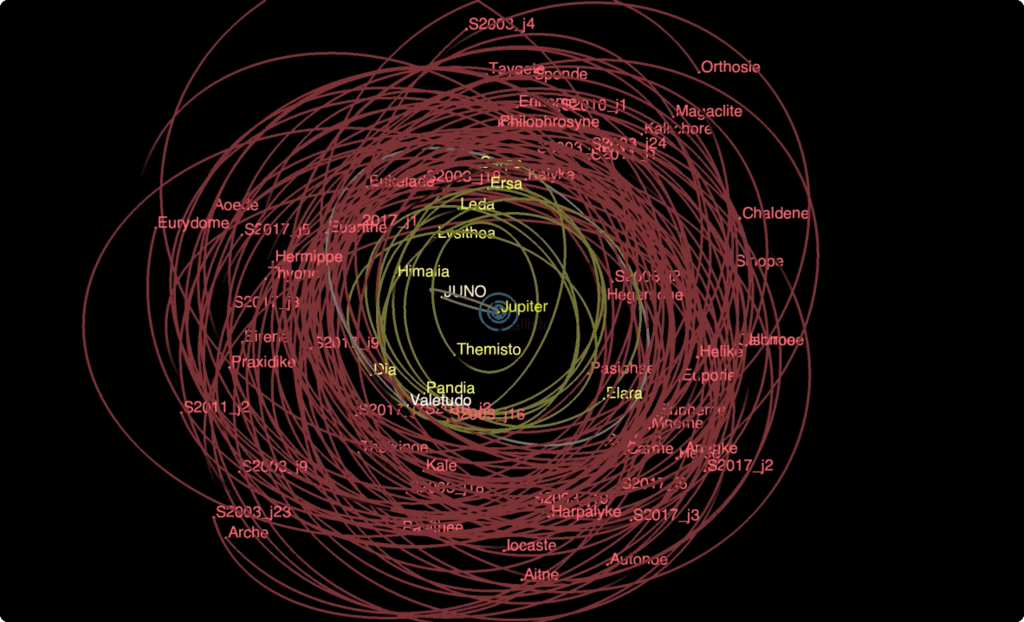
\includegraphics[width=0.95\textwidth, trim = {2cm, 0pt, 2cm, 0pt, clip}]{Examples/slide1_solar_system.png} % from: https://www.jpl.nasa.gov/events/moon-dance-exploring-the-moons-of-the-outer-solar-system
% 	\end{center}
% \end{columns}
% \end{frame}
\begin{frame}{Dynamical Systems}
	\vspace{-1cm}

	\begin{center}
		\includemovie[attach=false,autoplay,text={%
			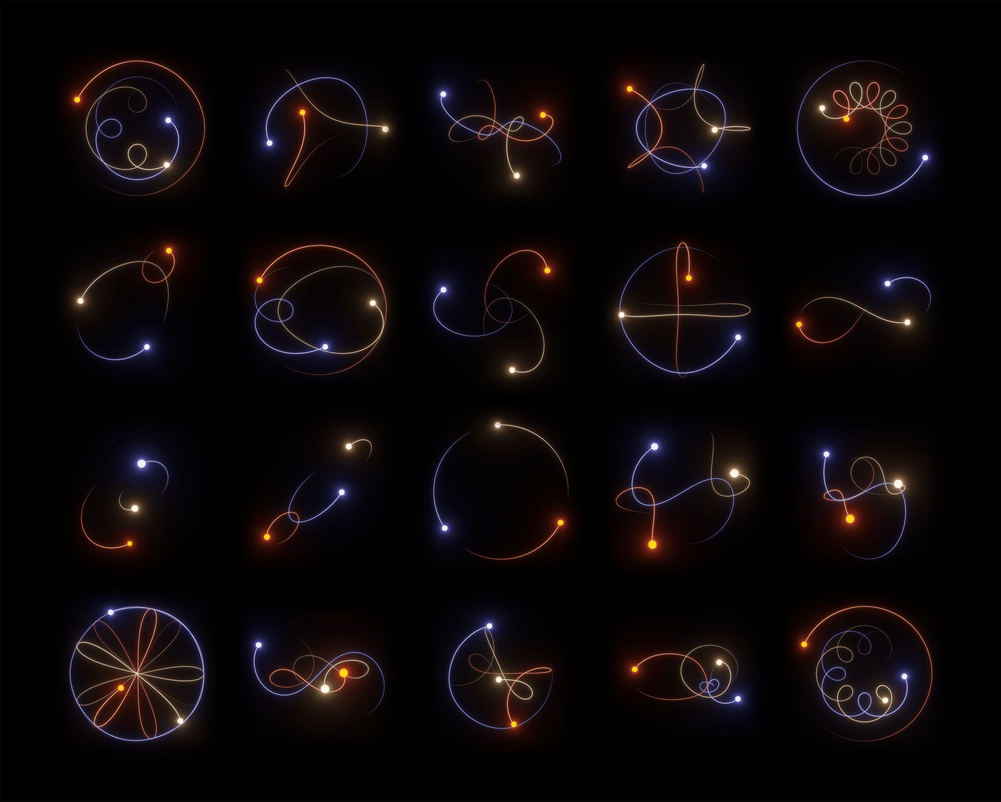
\includegraphics[width=0.55\textwidth]{Examples/three_body_problem.png}%
		  }]{0.55\linewidth}{0.55\linewidth}{images/Examples/three_body_problem.gif}
	  \end{center}

	  \nocite{3bodyproblemimage}
\end{frame}

\begin{frame}
\frametitle{Dynamical System $\to$ Behvaior}

\begin{columns}
	\column{0.3\textwidth}
		\[\begin{split}
			\dot x &= \sigma(y - x) \\
			\dot y &= x(\rho - z) - y \\
			\dot z &= xy - \beta z
		\end{split} \]
	\column{0.1\textwidth}
	\resizebox{1.5cm}{!}{$\longrightarrow$}
	\column{0.6\textwidth}
	\begin{center}
		
\includegraphics[width=0.95\textwidth, trim={4cm, 1.5cm, 4cm, 3cm}, clip]{Examples/slide3_lorenz_attractor.pdf}
	\end{center}
\end{columns}
\end{frame}

\begin{frame}
\frametitle{Data $\to$ Dynamical System}
\begin{columns}
	\column{0.6\textwidth}
	\begin{center}
		
\includegraphics[width=0.95\textwidth, trim={4cm, 1.5cm, 4cm, 3cm}, clip]{Examples/slide3_lorenz_attractor.pdf}
	\end{center}

	\column{0.1\textwidth}
	\resizebox{1.7cm}{!}{${? \atop \longrightarrow }$}
	\column{0.3\textwidth}
	\[ \frac{\mathrm d}{\mathrm dt} \mathbf x(t) = \mathbf f(\mathbf x(t)) \]
\end{columns}

\end{frame}



\section{SINDy}

\begin{frame}{Sparse Identification of Nonlinear Dynamics (SINDy)}

\begin{vfilleditems}
	\item[(1)] Collect data ($\mathbf X$) and derivatives ($\mathbf {\dot X}$)
	\item[(2)] Construct function library $\Theta(\mathbf X)$
	\item[(3)] Solve sparse regression problem $\mathbf {\dot X} = \Theta(\mathbf X) \mathbf \Xi$
\end{vfilleditems}
\end{frame}

\begin{frame}{Data}
	\[ \mathbf X = \begin{bmatrix}
		\mathbf x^T(t_1) \\ \mathbf x^T(t_2) \\ \vdots \\ \mathbf x^T(t_m)
	\end{bmatrix} = \begin{bmatrix}
		x_1(t_1) & x_2(t_1) & \cdots & x_n(t_1) \\
		x_1(t_2) & x_2(t_2) & \cdots & x_n(t_2) \\
		\vdots & \vdots & \ddots & \vdots \\ 
		x_1(t_m) & x_2(t_m) & \cdots & x_n(t_m)
	\end{bmatrix} \]
\end{frame}

\begin{frame}{Derivatives}
	\[ \mathbf {\dot X} = \begin{bmatrix}
		\mathbf {\dot x}^T(t_1) \\ \mathbf {\dot x}^T(t_2) \\ \vdots \\ \mathbf {\dot x}^T(t_m)
	\end{bmatrix} = \begin{bmatrix}
		\dot x_1(t_1) & \dot x_2(t_1) & \cdots & \dot x_n(t_1) \\
		\dot x_1(t_2) & \dot x_2(t_2) & \cdots & \dot x_n(t_2) \\
		\vdots & \vdots & \ddots & \vdots \\ 
		\dot x_1(t_m) & \dot x_2(t_m) & \cdots & \dot x_n(t_m)
	\end{bmatrix} \]
\end{frame}

\begin{frame}{Function Library}
	\[  \Theta(\mathbf X) = \begin{bmatrix} \mid & \mid & \mid & \mid &  & \mid & \mid & \\ 1 & \mathbf X & {\mathbf X}^{P_2} & {\mathbf X}^{P_3} & \cdots & \sin{(\mathbf X)} & \cos{(\mathbf X)} & \cdots \\ \mid & \mid & \mid & \mid & & \mid & \mid & \end{bmatrix}  \]
\end{frame}

\begin{frame}{Function Library}
	\[  \Theta(\mathbf X) = \begin{bmatrix} \mid & \mid & \mid & \mid &  & \mid & \mid & \\ 1 & \mathbf X & {\mathbf X}^{P_2} & {\mathbf X}^{P_3} & \cdots & \sin{(\mathbf X)} & \cos{(\mathbf X)} & \cdots \\ \mid & \mid & \mid & \mid & & \mid & \mid & \end{bmatrix}  \]

	\vspace{1.5em}

	\[ \mathbf X^{P_2} = \begin{bmatrix}
		x_1^2(t_1) & x_1(t_1)x_2(t_1) & \cdots & x_1(t_1)x_n(t_1) & x_2^2(t_1) & \cdots & x_n^2(t_1) \\
		x_1^2(t_2) & x_1(t_2)x_2(t_2) & \cdots & x_1(t_2)x_n(t_2) & x_2^2(t_2) & \cdots & x_n^2(t_2) \\
		\vdots & \vdots & \ddots & \vdots & \vdots & \ddots & \vdots \\
		x_1^2(t_m) & x_1(t_m)x_2(t_m) & \cdots & x_1(t_m)x_n(t_m) & x_2^2(t_m) & \cdots & x_n^2(t_m) \\
	\end{bmatrix} \]

\end{frame}

\begin{frame}{Function Library}
	\[  \Theta(\mathbf X) = \begin{bmatrix} \mid & \mid & \mid & \mid &  & \mid & \mid & \\ 1 & \mathbf X & {\mathbf X}^{P_2} & {\mathbf X}^{P_3} & \cdots & \sin{(\mathbf X)} & \cos{(\mathbf X)} & \cdots \\ \mid & \mid & \mid & \mid & & \mid & \mid & \end{bmatrix}  \]

	\vspace{1.5em}

	\[ \sin{(\mathbf X)} = \begin{bmatrix}
		\sin(x_1(t_1)) & \sin(x_2(t_1)) & \cdots & \sin(x_n(t_1)) \\ 
		\sin(x_1(t_2)) & \sin(x_2(t_2)) & \cdots & \sin(x_n(t_2)) \\
		\vdots & \vdots & \ddots & \vdots \\ 
		\sin(x_1(t_m)) & \sin(x_2(t_m)) & \cdots & \sin(x_n(t_m))
	\end{bmatrix} \]
\end{frame}

\begin{frame}{Function Library}
	\[ \dot x_i(t) = f_i(\mathbf x(t)) = a_1g_1(\mathbf x(t)) + a_2 g_2(\mathbf x(t)) + \cdots + a_k g_k(\mathbf x(t)) \]
	\pause
	\vspace{1.5em}

	\[ \Theta(\mathbf X) = \begin{bmatrix}
		g_1(\mathbf x(t_1)) & g_2(\mathbf x(t_1)) & \cdots & g_k(\mathbf x(t_1)) \\
		g_1(\mathbf x(t_2)) & g_2(\mathbf x(t_2)) & \cdots & g_k(\mathbf x(t_2)) \\ 
		\vdots & \vdots & \ddots & \vdots \\ 
		g_1(\mathbf x(t_m)) & g_2(\mathbf x(t_m)) & \cdots & g_k(\mathbf x(t_k))
	\end{bmatrix} \]
\end{frame}

\begin{frame}{Sparse Regression}
	\[ \scalebox{2}{$\mathbf {\dot X} = \Theta(\mathbf X)\mathbf \Xi$} \]

	\vspace{2em}

	\[ \mathbf \Xi = \begin{bmatrix} \boldsymbol \xi_1 & \boldsymbol \xi_2 & \cdots & \boldsymbol \xi_n \end{bmatrix}  \]
\end{frame}

\begin{frame}[fragile]
	\frametitle{Sparse Regression}

	\begin{lstlisting}[language = Julia]
function sparse_regression(Theta, Xdot, lambda, kmax) 
    Xi = Theta\Xdot # create initial guess for Xi as just regression
    for _ in 1:kmax 
        # find coefficients that are less than lambda
        small_coefficients = abs.(Xi) .< lambda
        Xi[small_coefficients] .= 0 # set small coefficients to 0 

        # now individually run regression on non-zero coefficients
        for n in 1:(size(Xdot)[2]) # loop through all state dimensions 
            nonsmall = .!small_coefficients[:, n]
            
            Xi[nonsmall, n] = Theta[:, nonsmall]\Xdot[:, n]
        end # for n
    end # for k 
    Xi
end # function sparse_regression
	\end{lstlisting}
\end{frame}

\begin{frame}{Sparse Regression Result}
	\[ \mathbf \Xi = \begin{bmatrix}
		\mathbf \xi_1 & \mathbf \xi_2 & \cdots & \mathbf \xi_n
	\end{bmatrix} \]

	% \vspace{1.5em}
	\[ \mathbf \xi_i = \begin{bmatrix}
		\xi_{i, 1} \\ \xi_{i, 2} \\ \vdots \\ \xi_{i, k}
	\end{bmatrix} \quad \implies \quad \dot x_i(t) = \xi_{i, 1}g_1(\mathbf x(t)) + \xi_{i, 2}g_2(\mathbf x(t)) + \cdots + \xi_{i, k}g_k(\mathbf x(t)) \]

	\[ \text{Most } \xi_{i, j} = 0. \]
\end{frame}

\section{Results}

\begin{frame}{Lorenz System}
	\begin{columns}
		\column{0.35\textwidth}
		\[\begin{split}
			\dot x &= \sigma(y - x) \\
			\dot y &= x(\rho - z) - y \\
			\dot z &= xy - \beta z
		\end{split} \]
		\column{0.65\textwidth}
		\begin{center}
			
\includegraphics[width=0.95\textwidth, trim={4cm, 1.5cm, 4cm, 3cm}, clip]{Examples/slide3_lorenz_attractor.pdf}
		\end{center}
	\end{columns}
\end{frame}

% \begin{frame}{Found Lorenz System ($\eta = 0.01$)}
% 	\begin{columns}
% 		\column{0.35\textwidth}
% 			\[ \begin{split}
% 				\dot x &= -9.947x + 9.976y \\
% 				\dot y &= 27.041x -0.669y -0.976xz \\
% 				\dot z &= -2.650z + 0.996xy
% 			\end{split} \]
% 			{\small Normalized derivative distance: $0.0175$}
% 			\vspace{0.2em }

% 			{\small \begin{multline*}\mathcal B = \{ \mathbf 1, \mathbf X, \mathbf X^{P_2}, \ldots, \mathbf X^{P_7}, \\ \sin{(\mathbf X)}, \ldots, \sin{(10\mathbf X)}, \\ \cos{(\mathbf X)}, \cos{(10\mathbf X)} \} \end{multline*}
% 			}
% 			% \resizebox{1.5\textwidth}{!}{ \begin{multline}\mathcal B = \\ \{ \mathbf 1, \mathbf X^{P_1}, \ldots, \mathbf X^{P_7}, \\ \sin{(\mathbf X)}, \ldots, \sin{(10\mathbf X)}, \cos{(\mathbf X)}, \cos{(10\mathbf X)} \} \end{multline}}
% 			% \pause 
% 			% \[
% 			% \begin{split}
% 			% 	\dot x &= -10x + 10 y \\ 
% 			% 	\dot y &= 27x - y - xz \\ 
% 			% 	\dot z &= 
% 			% \end{split}	
% 			% \]
% 		\column{0.65\textwidth}
% 		\begin{center}
% 			
\includegraphics[width=0.95\textwidth, trim={4cm, 1.5cm, 4cm, 3cm}, clip]{found_lorenz_001.pdf}
% 		\end{center}
% 	\end{columns}
% \end{frame}

% \begin{frame}{Found Lorenz System ($\eta = 0.1$)}
% 	\begin{columns}
% 		\column{0.35\textwidth}
% 			\[ \begin{split}
% 				\dot x &= -9.806x + 9.838y \\
% 				\dot y &= 25.912x -0.433y  -0.946xz \\
% 				\dot z &= -2.613z + 0.982xy
% 			\end{split} \]
% 			{\small Normalized derivative distance: $0.0469$}
% 			\vspace{0.2em}

% 			{\small \begin{multline*}\mathcal B = \{ \mathbf 1, \mathbf X, \mathbf X^{P_2}, \ldots, \mathbf X^{P_5}, \\ \sin{(\mathbf X)}, \ldots, \sin{(10\mathbf X)}, \\ \cos{(\mathbf X)}, \cos{(10\mathbf X)} \} \end{multline*}
% 			}
% 			% \pause 
% 			% \[
% 			% \begin{split}
% 			% 	\dot x &= -10x + 10 y \\ 
% 			% 	\dot y &= 27x - y - xz \\ 
% 			% 	\dot z &= 
% 			% \end{split}	
% 			% \]
% 		\column{0.65\textwidth}
% 		\begin{center}
% 			
\includegraphics[width=0.95\textwidth, trim={4cm, 1.5cm, 4cm, 3cm}, clip]{found_lorenz_01.pdf}
% 		\end{center}
% 	\end{columns}
% \end{frame}
% \begin{frame}{Found Lorenz System ($\eta = 1$)}
% 	\begin{columns}
% 		\column{0.35\textwidth}
% 			\[ \begin{split}
% 				\dot x &= -7.004x + 7.144y \\
% 				\dot y &= 14.982x + 1.537y -0.635xz \\
% 				\dot z &=-2.153 -2.151z + 0.839xy
% 			\end{split} \]
% 			{\small Normalized derivative distance: $0.2973$}
% 			\vspace{0.2em}

% 			{\small \[\mathcal B = \{ \mathbf 1,\mathbf X, \mathbf X^{P_2}, \ldots, \mathbf X^{P_5} \} \]
% 			}
% 			% \pause 
% 			% \[
% 			% \begin{split}
% 			% 	\dot x &= -10x + 10 y \\ 
% 			% 	\dot y &= 27x - y - xz \\ 
% 			% 	\dot z &= 
% 			% \end{split}	
% 			% \]
% 		\column{0.65\textwidth}
% 		\begin{center}
% 			
\includegraphics[width=0.95\textwidth, trim={4cm, 1.5cm, 4cm, 3cm}, clip]{found_lorenz_1.pdf}
% 		\end{center}
% 	\end{columns}
% \end{frame}

\begin{frame}{Found Lorenz Systems}
	\begin{columns}
		\column{0.25\textwidth}
			\[ \text{Actual} \]
			\begin{center}
				
\includegraphics[width=0.95\textwidth, trim={4cm, 3.2cm, 4cm, 3.1cm}, clip]{Examples/slide3_lorenz_attractor.pdf}
			\end{center}
			\begin{equation*}
				\resizebox{!}{1.4em}{ $\begin{aligned}
				\dot x &= 10(y - x) \\
				\dot y &= x(28 - z) - y \\
				\dot z &= xy - (8/3) z
				\end{aligned} $}
			\end{equation*}
			\[\text{\small $\phantom{E_\text{der} = 0.00136}$}\]
		\column{0.25\textwidth}
		\[ \eta = 0.01 \]
		\begin{center}
			
\includegraphics[width=0.95\textwidth, trim={4cm, 3.2cm, 4cm, 3.1cm}, clip]{found_lorenz_001.pdf}
		\end{center}
		\begin{equation*}
		\resizebox{!}{1.4em}{ $\begin{aligned}
			\dot x &=  9.976y-9.947x \\
			\dot y &= 27.041x  -0.976xz-0.669y \\
			\dot z &=  0.996xy - 2.650z
		\end{aligned} $}
		\end{equation*}
		\[ \text{\small $E_{\text{der}} = 0.00136$} \]

		\column{0.25\textwidth}
		\[ \eta = 0.1 \]
		\begin{center}
			
\includegraphics[width=0.95\textwidth, trim={4cm, 3.2cm, 4cm, 3.1cm}, clip]{found_lorenz_01.pdf}
		\end{center}
		\begin{equation*}
		\resizebox{!}{1.4em}{$\begin{aligned}
			\dot x &=   9.838y -9.806x\\
			\dot y &= 25.912x   -0.946xz-0.433y \\
			\dot z &=   0.982xy-2.613z
		\end{aligned} $}
		\end{equation*}
		\[ \text{\small $E_\text{der} = 0.00349$} \]

		\column{0.25\textwidth}
		\[ \eta = 1 \]
		\begin{center}
			
\includegraphics[width=0.95\textwidth, trim={4cm, 3.2cm, 4cm, 3.1cm}, clip]{found_lorenz_1.pdf}
		\end{center}
		\begin{equation*}
		\resizebox{!}{1.4em}{$ \begin{aligned}
			\dot x &=  7.144y-7.004x \\
			\dot y &= 14.982x  -0.635xz+ 1.537y \\
			\dot z &=   0.839xy-2.151z-2.153
		\end{aligned} $}
		\end{equation*}
		\[ \text{\small $E_\text{der} = 0.10119$} \]
	\end{columns}
\end{frame}

\begin{frame}{SINDy and Bifurcations}
	\begin{equation*}
		\begin{split}
			\mathbf {\dot x} &=  \mathbf{f}(\mathbf x; \mu) \\
			\dot \mu &= 0
		\end{split}
	\end{equation*}

	\vspace{1.5em}

	\[ \mathbf X = \begin{bmatrix}
		\mathbf X_{\mu_0} \\ \mathbf X_{\mu_1} \\ \vdots \\ \mathbf X_{\mu_h}
	\end{bmatrix} \]
\end{frame}

\begin{frame}{The Hopf Normal Form}
	\begin{columns}
		\column{0.35\textwidth}
		\begin{equation*}
			\resizebox{\textwidth}{!}{$
			\begin{aligned}
				\dot x &= \mu x - \omega y - Ax(x^2 + y^2) \\
			\dot y &= \omega x +\mu y - Ay(x^2 + y^2)
			\end{aligned}
			$}
		\end{equation*}
		\column{0.65\textwidth}
		\begin{center}
			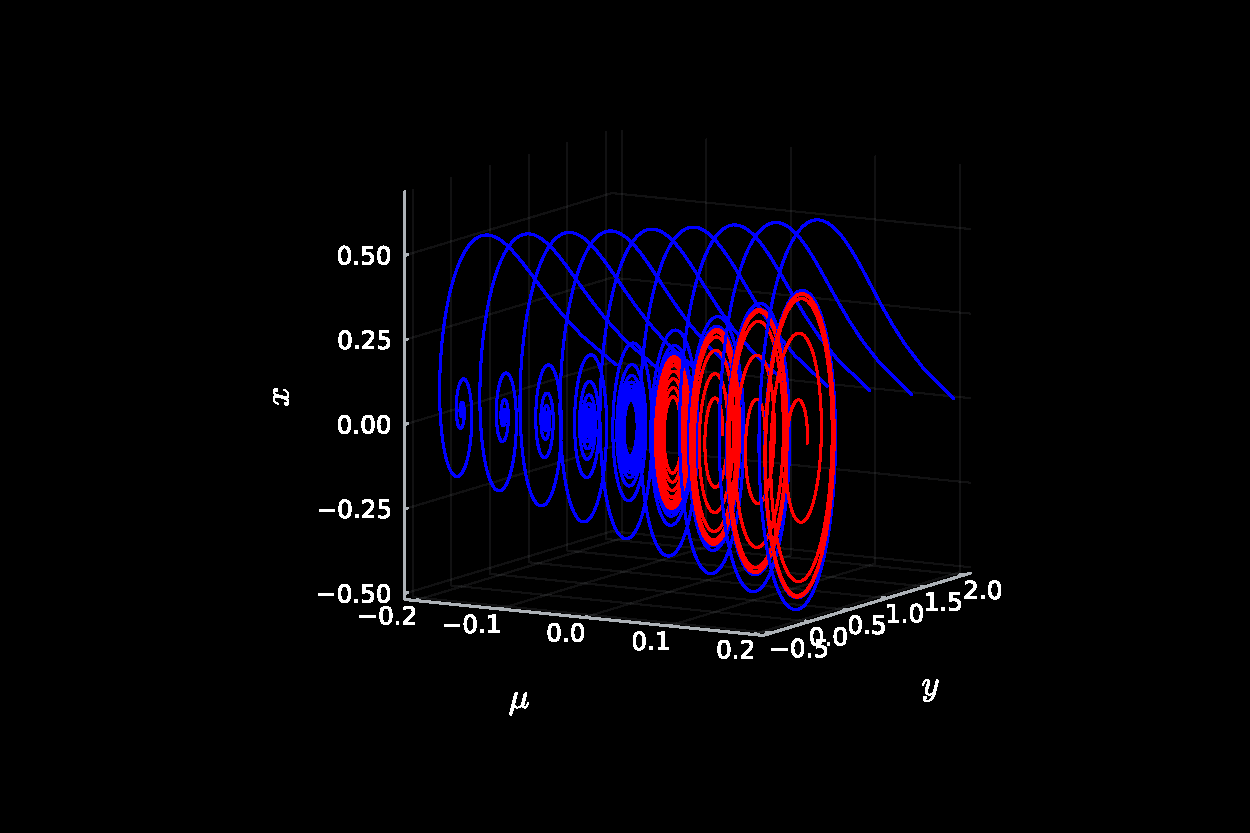
\includegraphics[width=0.85\textwidth, trim = {4cm, 2cm, 4cm, 2.5cm}, clip]{hopf_normal_actual.pdf}
		\end{center}
	\end{columns}
\end{frame}

\begin{frame}{Found Hopf Bifurcation}
	\begin{columns}
		\column{0.5\textwidth}
		\[ \text{Actual} \]
		\begin{center}
			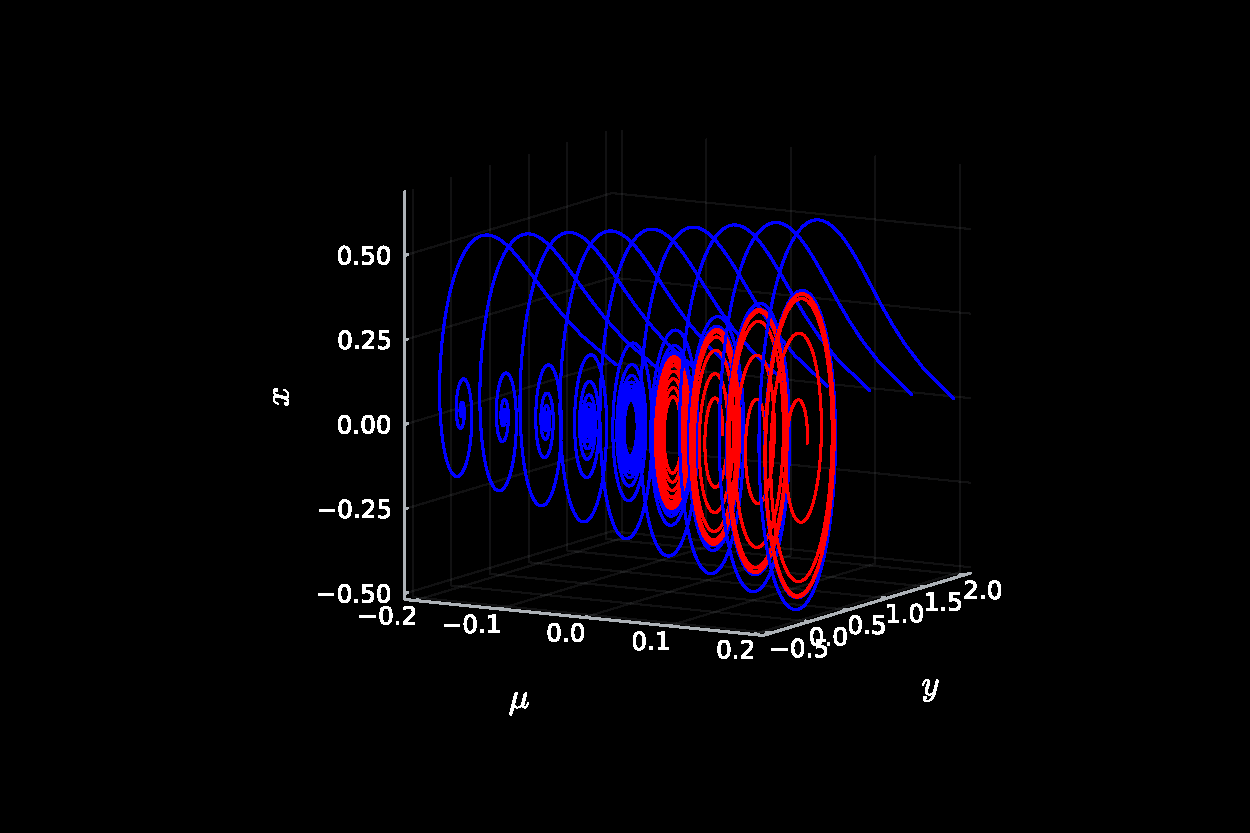
\includegraphics[width=0.7\textwidth, trim = {4cm, 2cm, 4cm, 2.5cm}, clip]{hopf_normal_actual.pdf}
		\end{center}
		\begin{equation*}
			\resizebox{!}{1.2em}{$
			\begin{aligned}
			\dot x &= \mu x - y - x(x^2 + y^2) \\
			\dot y &= x + \mu y - y(x^2 + y^2) \\
			&\phantom{+ 0.769\mu xy^2 -0.723 \mu^2 x^2y} 
			\end{aligned}
			$}
		\end{equation*}
		\[\text{\small $\phantom{E_\text{der} = 0.00136}$}\]
		\column{0.5\textwidth}
		\[ \eta = 0.005 \]
		\begin{center}
			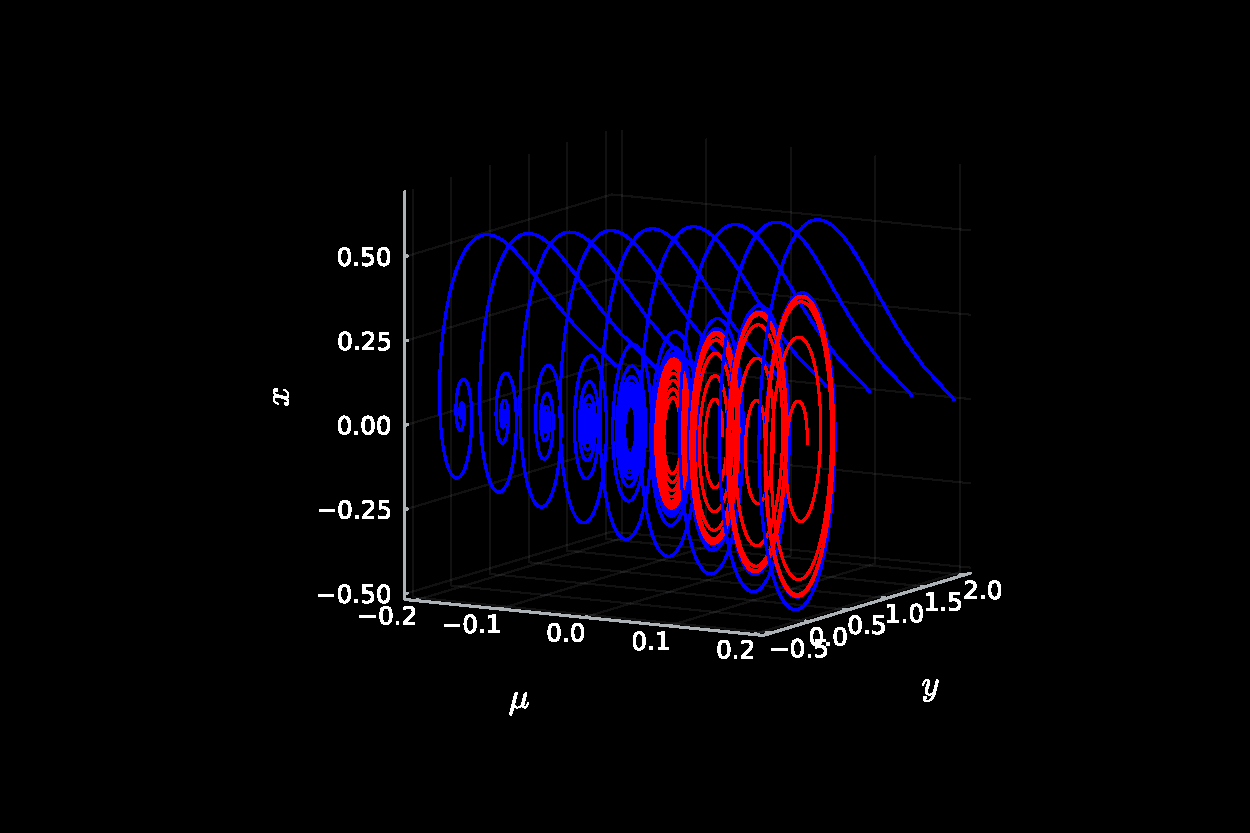
\includegraphics[width=0.7\textwidth, trim = {4cm, 2cm, 4cm, 2.5cm}, clip]{found_hopf_bifurcation_0005.pdf}
		\end{center}
		\begin{equation*}
			\resizebox{!}{1.2em}{$
			\begin{aligned}
				\dot x &= -0.957y + 0.908\mu x -0.888x^3 -1.303xy^2 \\
				&\quad  + 0.769\mu xy^2 -0.723 \mu^2 x^2y \\ 
				\dot y &= 0.966x + 0.961\mu y -0.927yx^2 - 0.962y^3
			\end{aligned}
			$}
		\end{equation*}
		\[\text{\small $E_\text{der} = 2.682 \times 10^{-6}$}\]
	\end{columns}
\end{frame}

\section{Conclusion}
\begin{frame}{Concluding Thoughts}
	\begin{vfilleditems}
		\item SINDy demonstrates performance in qualitative dynamics recovery 
		\item Concerns over stability with noise and parameters (how do we choose good basis/parameters?)
		\item Active learning?
	\end{vfilleditems}
\end{frame}

\begin{frame}{Citations}
	\nocite{sindy}
	
	\printbibliography

	\vfill
\end{frame}

\end{document}